% TeX root = ../Main.tex

% First argument to \section is the title that will go in the table of contents. Second argument is the title that will be printed on the page.
\section[Lecture 1 -- {\it Kinematic Calibration}]{Kinematic Calibration}

\subsection{Introduction}

For a robot manipulator in a given configuration, the actual values of the task-space variables may slightly
deviate from those computed via direct kinematics. Thus it may lead to a deviation between the end-effector pose
reached in a given configuration and the pose compute via direct kinematics. Such deviations characterize the
\textit{accuracy} of a robot manipulator (its ability to reproduce precisely the commanded pose in task space).
The accuracy is different from \textit{repeatability}, which is the robot capability to reproduce exactly the 
same commanded pose in more attempts. It depends more on the mechanical components' and control loops' quality.

The positional accuracy error may be reduced drastically by using the \textbf{kinematic calibration procedure}.
The reasons why calibration is crucial in real-world conditions can be summarized by three principal problems:

\begin{itemize}[noitemsep]
  \item Mechanical tolerances;
  \item Encoder offsets (bias which make inconsistent the ``zero reference'' of the robot);
  \item Open kinematic chain loop (which amplifies the errors distributed along the arm).
\end{itemize}

Mathematically, let $\mathbf{y}_{e, nom} = \mathbf{k}_{e}(\boldsymbol{\alpha}, \mathbf{a}, \mathbf{d}, \boldsymbol{\theta})$
be the nominal Direct Kinematics (DK) mapping the joint space $\mathbf{q}$ to the task space $\mathbf{y}$, with constant geometric parameters. The calibration task consists of finding the true parameter values to decrease the discrepancy between the measured pose $\mathbf{y}_{e}$ and the nominal pose $\mathbf{y}_{e, nom}$:
$$
\Delta y_e = y_e - y_{e,nom} = \frac{\partial k_e}{\partial \alpha} \cdot \Delta \alpha + \frac{\partial k_e}{\partial a} \cdot \Delta a + \frac{\partial k_e}{\partial d} \cdot \Delta d + \frac{\partial k_e}{\partial \theta} \cdot \Delta \theta
$$

In the equation, the partial derivatives represent the partial Jacobians evaluated in nominal conditions and 
are multiplied by the first-order variations of the DH table values.

\subsection{Calibration Procedure}
To rewrite the linearization in a more compact matrix form, 
let's define the parameter variation vector $\Delta \varphi$ (of dimension $4n \times 1$) 
and the Jacobian matrix $\Phi$ (of dimension $6 \times 4n$, assuming full pose data):

$$
\Delta \varphi = 
\begin{pmatrix}
\Delta \alpha \\
\Delta a \\
\Delta d \\
\Delta \theta
\end{pmatrix}, \quad
\Phi = 
\begin{pmatrix}
\frac{\partial k_e}{\partial \alpha} & \frac{\partial k_e}{\partial a} & \frac{\partial k_e}{\partial d} & \frac{\partial k_e}{\partial \theta}
\end{pmatrix}
$$

This allows us to express the single-pose calibration equation as:
$$
\Delta y_e = \Phi \Delta \varphi
$$

Since a single measurement is not enough to identify all the parameters, 
we need to perform $\ell$ experiments (with $\ell \gg n$). By stacking the measured pose errors and 
the corresponding matrices evaluated at different nominal configurations, we obtain:

$$
\overline{\Delta y_e} = 
\begin{pmatrix}
\Delta y_{e,1} \\
\Delta y_{e,2} \\
\vdots \\
\Delta y_{e,\ell}
\end{pmatrix}_{6\ell \times 1}, \quad
\overline{\Phi} = 
\begin{pmatrix}
\Phi_1 \\
\Phi_2 \\
\vdots \\
\Phi_\ell
\end{pmatrix}_{6\ell \times 4n}
$$

The overall calibration equation for multiple experiments becomes a linear system:
$$
\overline{\Delta y_e} = \overline{\Phi} \Delta \varphi
$$

In this final system:
\begin{itemize}[noitemsep]
    \item $\overline{\Delta y_e}$ is the vector obtained from measurements;
    \item $\overline{\Phi}$ is the \textbf{regressor matrix} evaluated at nominal parameters. For the system to be solvable, this matrix must have full column rank (achievable for a sufficiently large $\ell$);
    \item $\Delta \varphi$ is the vector of unknowns we want to estimate.
\end{itemize}

\subsection{Calibration Algorithm}

The overall calibration equation $\overline{\Delta y_e} = \overline{\Phi} \Delta \varphi$ represents
a linearized least squares problem. 
Since the true direct kinematics function is non-linear, this linearized formulation needs an iterative solution, 
dictated by the following algorithm:

% Inizializzazione allineata a sinistra
\begin{flalign*}
    &\epsilon_r = 10^{-4}, \quad i_{max} = 50 & \\
    &\varphi^{(0)} = \varphi_{nom} & \\
    &\overline{\Phi}^{(0)} = \overline{\Phi}(\varphi^{(0)}) & \\
    &\overline{\Delta y_e}^{(0)} = \overline{\Delta y_e}(\varphi^{(0)}) & \\
    &i = 0 &
\end{flalign*}

% Ciclo iterativo
\noindent \textbf{if} $\left\| \overline{\Delta y_e}^{(i)} \right\| \le \epsilon_r$
\begin{itemize}[label={}, leftmargin=2em, nosep]
    \item $\varphi^* = \varphi^{(i)} \quad \leftarrow \text{\textit{final solution}}$
\end{itemize}
\textbf{else if} $i \le i_{max}$
\begin{itemize}[label={}, leftmargin=2em, nosep]
    \item $\Delta \varphi^{(i)} = \left(\overline{\Phi}^{(i)}\right)^\# \overline{\Delta y_e}^{(i)} = \left( {\overline{\Phi}^{(i)}}^T \overline{\Phi}^{(i)} \right)^{-1} {\overline{\Phi}^{(i)}}^T \overline{\Delta y_e}^{(i)}$
    \item $\varphi^{(i+1)} = \varphi^{(i)} + \Delta \varphi^{(i)}$
    \item $\overline{\Phi}^{(i+1)} = \overline{\Phi}(\varphi^{(i+1)})$
    \item $\overline{\Delta y_e}^{(i+1)} = \overline{\Delta y_e}(\varphi^{(i+1)})$
    \item $i = i + 1$
\end{itemize}
\textbf{else}
\begin{itemize}[label={}, leftmargin=2em, nosep]
    \item \texttt{disp('no convergence in $i_{max}$ iterations')}
\end{itemize}
\textbf{end if}

\vspace{1em}

\subsubsection*{Algorithm Breakdown}
To better understand the iterative procedure, we can break it down into the following key steps:

\begin{enumerate}
    \item \textbf{Initialization:} We define a tolerance threshold ($\epsilon_r$) and a maximum number of iterations ($i_{max}$) to prevent infinite loops. We start by guessing that our parameters are equal to the nominal ones ($\varphi^{(0)} = \varphi_{nom}$).
    \item \textbf{Convergence Check:} At each step $i$, we evaluate the norm of the pose error $\left\| \overline{\Delta y_e}^{(i)} \right\|$. If this error is smaller than our tolerance $\epsilon_r$, the algorithm stops, and the current parameters are accepted as the true calibrated parameters $\varphi^*$.
    \item \textbf{Least Squares Minimization:} If the error is still too large, we compute the required parameter variation $\Delta \varphi^{(i)}$. Since the matrix $\overline{\Phi}$ is rectangular (overdetermined system), we use the \textbf{Moore-Penrose pseudoinverse} $\left(\overline{\Phi}^{(i)}\right)^\#$. This specific mathematical operation finds the $\Delta \varphi^{(i)}$ that minimizes the squared error norm $\left\| \overline{\Phi}^{(i)}\Delta \varphi - \overline{\Delta y_e}^{(i)} \right\|^2$.
    \item \textbf{Update Rule:} The calculated variation $\Delta \varphi^{(i)}$ is added to the current parameters to generate a new, more accurate guess $\varphi^{(i+1)}$. This new set contains the updated Denavit-Hartenberg parameters and the newly estimated encoder offsets (bias on $\theta$).
    \item \textbf{Re-evaluation:} The regressor matrix $\overline{\Phi}$ and the pose error $\overline{\Delta y_e}$ are re-evaluated using the newly found parameters $\varphi^{(i+1)}$, and the loop repeats.
\end{enumerate}

\subsection{Under- and Over-determined Systems}
Different solutions may be found when considering \textbf{Under-determined} and \textbf{Over-determined} 
systems of equations.

In the context of the calibration algorithm, we evaluate linear systems in the standard form $Ax = b$. 
For our calibration, the system is $\overline{\Phi} \Delta \varphi = \overline{\Delta y_e}$. 
Depending on the number of equations versus the number of unknowns, we face two different scenarios. 
Both are solved using the \textbf{Moore-Penrose pseudoinverse} $A^\#$:

\begin{figure}[H]
    \centering
    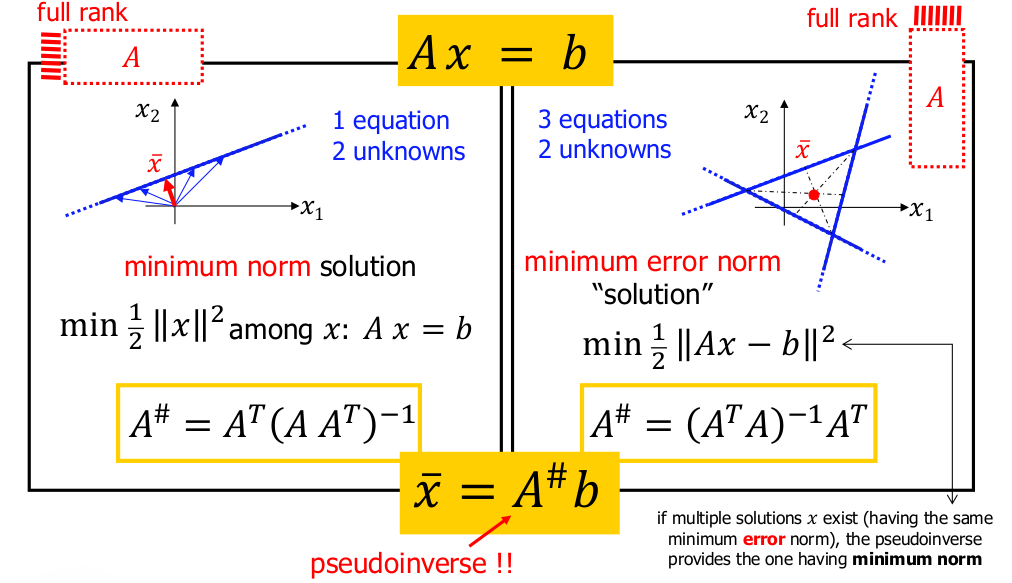
\includegraphics[width=1\textwidth]{Images/Calibration1.png}
    \caption{Geometric interpretation of under-determined and over-determined linear systems.}
    \label{fig:pseudoinverse}
\end{figure}

As illustrated in Figure \ref{fig:pseudoinverse}, the pseudoinverse handles two main configurations:

\begin{itemize}
    \item \textbf{Under-determined system (left):} There are fewer equations than unknowns (e.g., 1 equation, 2 unknowns). 
    The matrix $A$ has \textit{full row rank}. Since there are infinite exact solutions, 
    we look for the \textbf{minimum norm} solution, which minimizes $\frac{1}{2}\|x\|^2$ among all $x$ 
    such that $Ax = b$. The pseudoinverse used is:
    $$ A^\# = A^T(A A^T)^{-1} $$
    
    \item \textbf{Over-determined system (right):} There are more equations than unknowns (e.g., 3 equations, 2 unknowns). 
    The matrix $A$ has \textit{full column rank}. Because measurements contain noise, 
    an exact intersection usually does not exist. Instead, we look for the \textbf{minimum error norm} solution, 
    minimizing the squared error $\frac{1}{2}\|Ax - b\|^2$. The pseudoinverse used is:
    $$ A^\# = (A^T A)^{-1} A^T $$
\end{itemize}

In both scenarios, the optimal solution is compactly written as:
$$ \bar{x} = A^\# b $$
\textit{Note:} If multiple solutions exist with the same minimum error norm, the pseudoinverse automatically provides the one having the \textbf{minimum norm}.

\vspace{1em}
\noindent \textbf{Connection to Calibration:} 
Since we perform $\ell$ experiments where $\ell \gg n$, our calibration problem falls strictly into the \textbf{over-determined} category.
This justifies why our iterative algorithm calculates the parameter variation using the left-pseudoinverse formulation:
$\Delta \varphi^{(i)} = \left( {\overline{\Phi}^{(i)}}^T \overline{\Phi}^{(i)} \right)^{-1} {\overline{\Phi}^{(i)}}^T \overline{\Delta y_e}^{(i)}$.


\subsection{Final Comments}
The kinematic calibration procedure is an iterative least squared method, which starts as a non-linear problem
and it is linearized by using the first-order Taylor expansion. It represent an important problem in modern Robotics,
to accurate calibrate and estimate real parameters for sensors and model is foundamental to increase accuracy.